\section{Wireless}

Prima di passare alla configurazione vera e propria di tale rete, bisogna identificare le componenti che faranno parte della rete. I dispositivi sono gli stessi di una normale rete LAN a differenza del router che è di tipologia WRT300N, ovvero un wireless router. È possibile selezionare in Cisco Packet Tracer Student questo tipo di router cliccando in basso a sinistra sull’icona con l’etichetta “Wireless Device” e selezionare il router WRT300N.

\begin{center}
    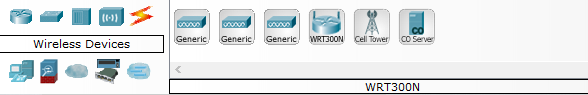
\includegraphics[width=\linewidth]{images/08.wireless/01.png}
\end{center}

Questo tipo router permetterà a tutti i dispositivi con modulo “WMP300N” di poter collegarsi collegare al router e utilizzare la rete. Tutti i dispositivi moderni come portatili, tablet e smartphone sono già dotati di questa tipologia di tecnologia potendoli già configurarli all’utilizzo della rete wireless.

\begin{center}
    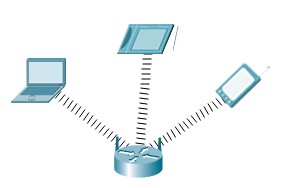
\includegraphics[width=0.4\linewidth]{images/08.wireless/02.png}
\end{center}

\subsection{Configurazione del modulo WPN300N}

Non tutti i computer hanno già in dotazione tale modulo, infatti computer di vecchia generazione non hanno la possibilità di collegarsi a reti wireless proprio per questo motivo. 

\begin{center}
    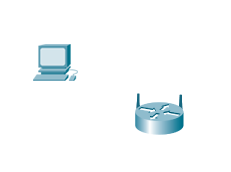
\includegraphics[width=0.4\linewidth]{images/08.wireless/03.png}
\end{center}

Per abilitarli ad utilizzare tali reti è necessario applicare alla loro interfaccia di rete proprio il modulo wireless. Per farlo bisognerà prima spegnere il computer stesso e verificare il tipo di modulo di rete applicato al computer.

\begin{center}
    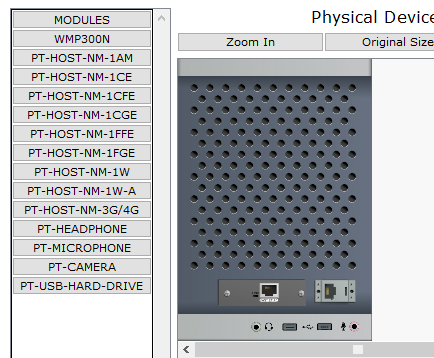
\includegraphics[width=0.5\linewidth]{images/08.wireless/04.png}
\end{center}

Una volta verificata la tipologia di modulo che è attualmente montato sul computer, bisognerà sostituirlo con quello di tipologia “WPN300N” e riaccendere il computer.

\begin{center}
    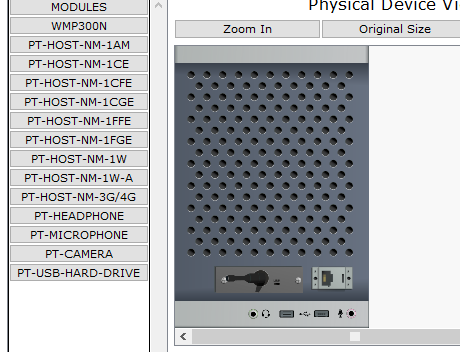
\includegraphics[width=0.5\linewidth]{images/08.wireless/05.png}
\end{center}

Effettuata questa serie di passaggi, il computer potrà captare tutte le connessioni wireless disponibili nella sua area e connettersi a quest’ultime, sfruttando i servizi di rete disponibili e accessibili.

\begin{center}
    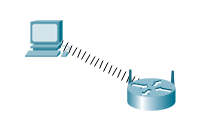
\includegraphics[width=0.4\linewidth]{images/08.wireless/06.png}
\end{center}

\subsection{Configurazione della rete}

Quindi come si configura una rete wireless? Come si è già fatto notare bisogna chiedersi se tutti dispositivi che si vogliono collegare alla rete possono effettivamente farlo, quindi controllare la loro interfaccia di rete (consultare il paragrafo “WPN300N” per vedere come si fa). Una volta verificata la percezione da parte degli host alla rete, bisognerà configurare quest’ultima in modo tale da potersi collegare e navigare in rete in modo sicuro ed efficiente.

\subsubsection{Wireless Router – Protocolli di sicurezza}

Di base, ogni wireless router, è sprovvisto di configurazioni wireless o protocolli di sicurezza nella sua interfaccia dando la possibilità a qualsiasi host di potersi collegare ad esso senza richiedergli nessun tipo di password o credenziale di accesso. In parole povere il wireless router è sprovvisto di chiave di sicurezza, pertanto ogni host che visualizzerà tale rete potrà connettersi senza problemi. L’assenza o meno della chiave può essere verificata nell’interfaccia “Config” del wireless router alla voce “Wireless”. Se all’interno di quest’ultima, nel campo “Authentication”, la spunta tra le varie opzioni sarà impostata su “Disabled” verrà confermata l’assenza della chiave.

\begin{center}
    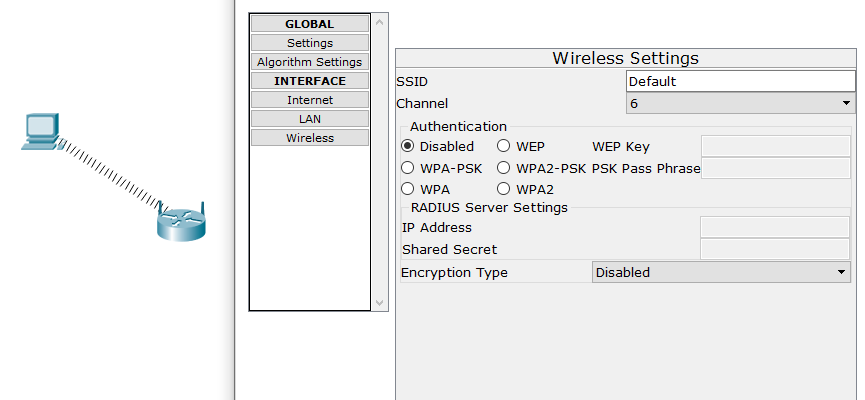
\includegraphics[width=\linewidth]{images/08.wireless/07.png}
\end{center}

Per ovviare a questo problema, bastera’ impostare un protocollo di sicurezza. Per fare cio’ bastera’ cliccare sopra il protocollo desiderato e soddisfare le richieste che richieste da quest’ultimo. Esistono diversi tipi di protocolli di sicurezza, in questo caso verranno analizzati soltanto quelli che vengono forniti dall’ambiente di sviluppo reti Cisco, ovvero:

\begin{itemize}
    \item WEP (Wired Equivalent Privacy): Questa tipologia di protocollo permette ai dispositivi nella rete di scambiarsi messaggi criptati, nascondendo cosi’ il contenuto dei messaggi a potenziali hacker o individui sospetti. Per poter accedere e utilizzare la rete, occorre sapere la chiave di sicurezza. Il protocollo WEP implementa una chiave la quale consiste in una sequenza di almeno dieci valori esadecimali. Per implementarla a livello pratico, dopo aver cliccato sopra la relativa combobox del protocollo, bastera’ inserire la chiave digitandola nella textbox recante etichetta “WEP Key”.\par
    \begin{center}
        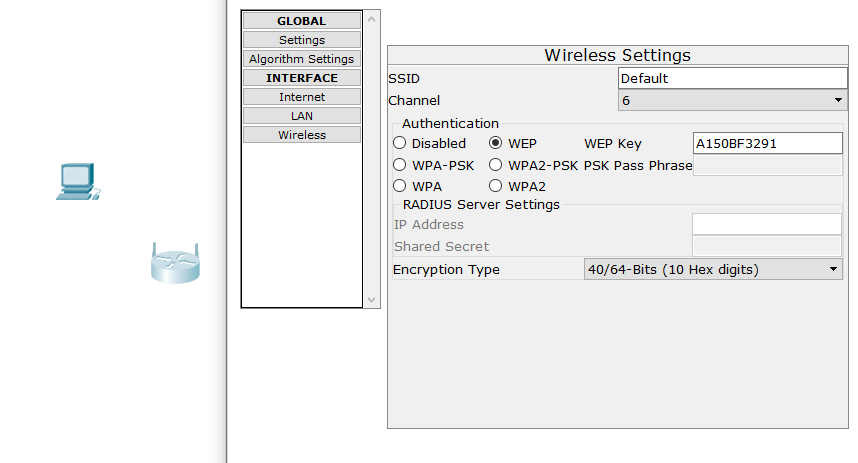
\includegraphics[width=\linewidth]{images/08.wireless/08.png}
    \end{center}

    \item WPA - PSK/WPA2 - PSK (WiFi Protected Access I e II – Pre Shared Key): Questo protocollo implementa un tipo specifico di sicurezza WPA nelle reti LAN domestiche le quali non richiedono uno specifico server di autentificazione (server Radius). Anche in questo caso per utilizzare e accedere alla rete occorre conoscere la chiave di sicurezza, la quale consiste in una vera e propria password di almeno 8 caratteri e massimo 63.  Questi due protocolli inoltre implementano due tipi diversi di protocolli di cifratura, ovvero il protocollo TKIP e il protocollo AES, fondamentali per la cifratura dei messaggi. Per implementare questo tipo di protocollo a livello pratico bisognera’ effettuare gli stessi identici passaggi spiegati nel WEP con l’unica differenza chge sta nella scelta del protocollo di cifratura.\par
    \begin{center}
        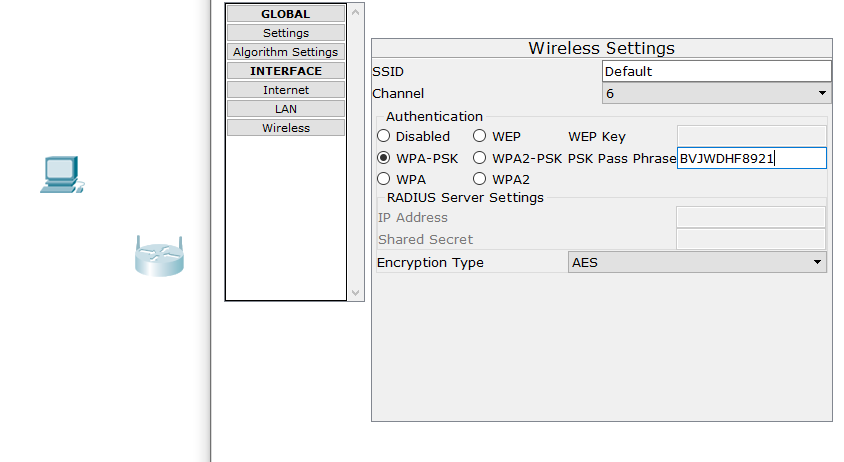
\includegraphics[width=\linewidth]{images/08.wireless/09.png}
    \end{center}

    \item WPA. (Wi-Fi Protected Access): Il WPA è un protocollo che nasce nel 2003 con lo scopo di facilitare la configurazione delle reti e di migliorare la sicurezza offerta.
    
    Il protocollo utilizzato per garantire la sicurezza è il TKIP (Temporal Key Integrity Protocol) che si basa sullo scambio di chiavi temporanee.

    Esistono due tipi di utilizzo del protocollo WPA:

    \begin{enumerate}
        \item WPA\_Personale: Questo tipo viene usato principalmente da piccoli uffici o a casa, non richiede un server di autenticazione e usa una chiave a 256 bit.
        \item WPA\_Impresa: Questo tipo viene usato principalmente nelle imprese e sfrutta un server RADIUS per la generazione automatica e l’autenticazione delle chiavi.
    \end{enumerate}
    
    \item WPA2 (Wi-Fi Protected Access 2): Il WPA2 rende sì ancora più facile la configurazione, ma soprattutto porta grandi migliorie per quanto riguarda la sicurezza.
    
    Di fatti il WPA2 usa l’algoritmo di cifratura AES (Advanced Encryption Standard).

    L’autenticazione avviene tramite il 4 way hand-shake.
\end{itemize}

L’implentazione pratica di questi due protocolli verrà approfondita a breve quando tratteremo le reti wireless con server Radius.

\subsection{Wireless Router – SSID}
Implementato il protocollo di sicurezza l’unica operazione rimasta da fare in modo tale da completare la configurazione del wireless router, è quella di assegnare alla rete un SSID. Un SSID non è altro che un identificativo che serve a distinguerla dalle altre reti wireless presenti nella zona, in modo tale che gli utenti possano subito riconoscerla in mezzo a tutte le altre. La procedura di assegnamento sarà molto semplice, infatti una volta aperta l’interfaccia “Config” del nostro wireless router, alla textbox recante etichetta “SSID” basterà sostituire il nome di default con quello scelto per la rete finale.

\begin{center}
    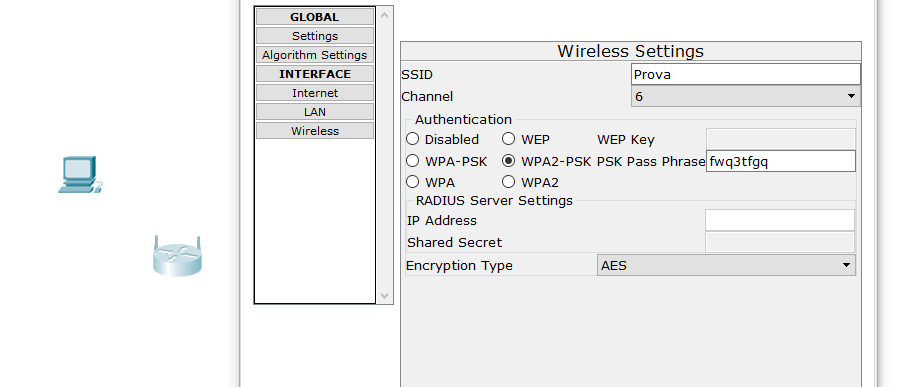
\includegraphics[width=\linewidth]{images/08.wireless/10.png}
\end{center}

Con questo ultimo passaggio si conclude la configurazione del wireless router.

\subsection{Host}
Come per il router, anche gli host hanno bisogno di essere configurati in modo tale da poter raggiungere la rete e comunicare attraverso essa, infatti di default anche l’host, come il router, è sprovvisto di configurazioni, che non interferirebbero troppo se anche il router ne fosse sprovvisto a sua volta. L’immagine riportata qui sotto rappresenta un host non configurato che tenta inutilmente di comunicare con il wireless router senza riuscirci proprio perché non è in grado di capirlo.

\begin{center}
    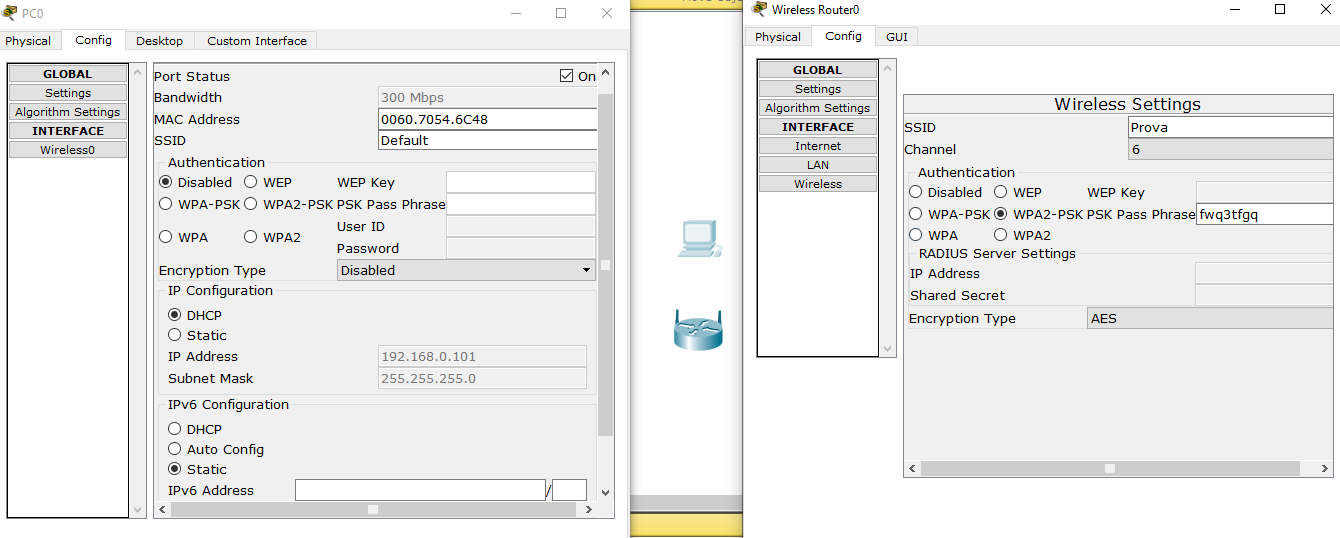
\includegraphics[width=\linewidth]{images/08.wireless/11.png}
\end{center}

Anche in questo caso tutte le configurazioni verranno effettuate all’interno dell’interfaccia “Config” del terminale host, nella sezione “Wireless”. Per fare in modo che l’host riesca a capire e a comunicare con il router, bisognerà impostare le stesse identiche configurazioni del router nell’interfaccia host, ovvero la SSID, il protocollo di sicurezza e il tipo di protocollo di cifratura (a parte con WEP). Le procedure di configurazione dell’host sono identiche a quelle del wireless router. Inseriti gli stessi dati di configurazione del router nell’host, quest’ultimo sarà in grado di comprendere e comunicare liberamente nella rete con il resto dei dispositivi connessi al wireless router.

\begin{center}
    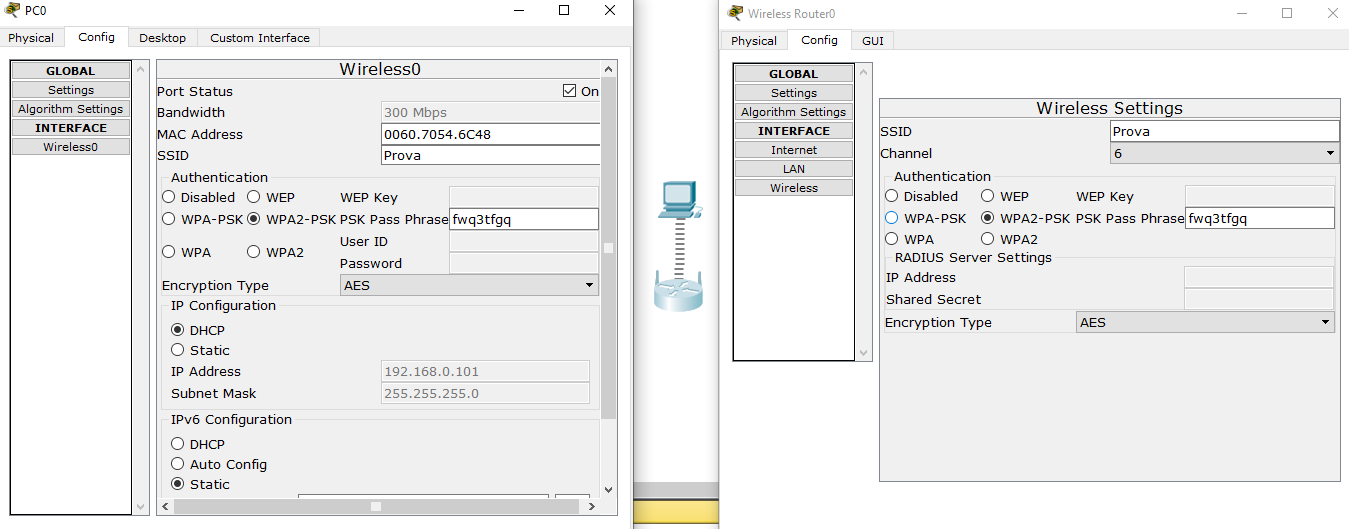
\includegraphics[width=\linewidth]{images/08.wireless/12.png}
\end{center}

\subsection{Comunicazione fra LAN o reti wireless diverse}
Le spiegazioni date nei paragrafi precedenti mostrano soltanto come far comunicare dispositivi nella stessa rete wireless, senza mostrare come tali comunicazioni si possano effettuare fra reti LAN o wireless diverse. Quindi come fare? Per prima cosa dobbiamo introdurre un nuovo dispositivo nella rete corrente, ovvero un router statico. Quest’ultimo è infatti indispensabile per stabilire comunicazioni fra reti diverse. Poi bisognerà collegare il wireless router direttamente con il router statico attraverso il cavo “Copper Straight-Through” nelle interfacce Ethernet dei due router.

\begin{center}
    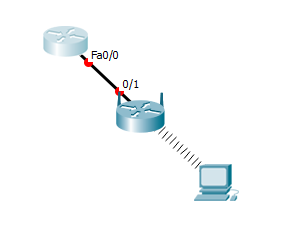
\includegraphics[width=0.4\linewidth]{images/08.wireless/13.png}
\end{center}

Fatto ciò bisognerà assegnare l’indirizzo che il router statico assumerà nella rete, attraverso il comando “Ip address” dandolo in input nell’interfaccia “CLI”.
Assegnato l’indirizzo al router ed effettuato il comando “no shutdown”, la via di comunicazione e le rispettive porte verranno attivate.

\begin{center}
    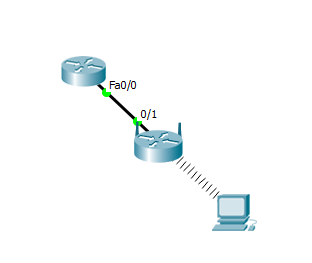
\includegraphics[width=0.4\linewidth]{images/08.wireless/14.png}
\end{center}

L’ultima operazione rimasta da eseguire è quella di configurare le interfacce “LAN” e “Internet” del wireless router. Nella prima interfaccia si andrà a definire l’indirizzo ip del wireless router nella sotterete wi-fi e dovrà essere settato in modo statico e manuale inserendolo nell’apposita textbox recante l’etichetta “IP address”.

\begin{center}
    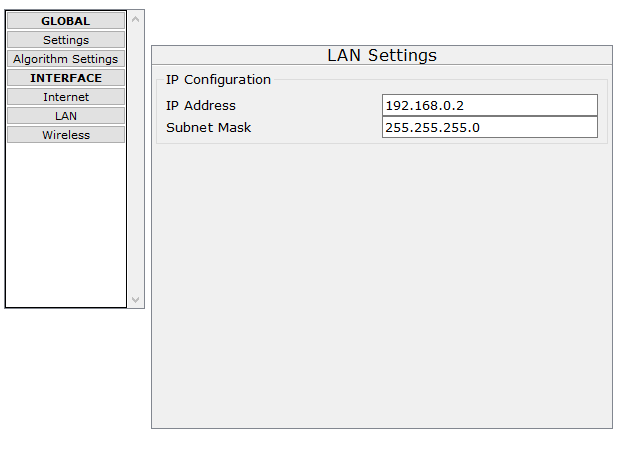
\includegraphics[width=\linewidth]{images/08.wireless/15.png}
\end{center}

L’ultima interfaccia invece permette al router wireless di poter comunicare con le altre reti andando a definire il default gateway, ovvero l’indirizzo IP che assume il router statico nella porta di comunicazione verso il wireless router. Per settarlo basterà, come per l’interfaccia LAN, inserire manualmente l’indirizzo IP del default gateway nella relativa textbox.

\begin{center}
    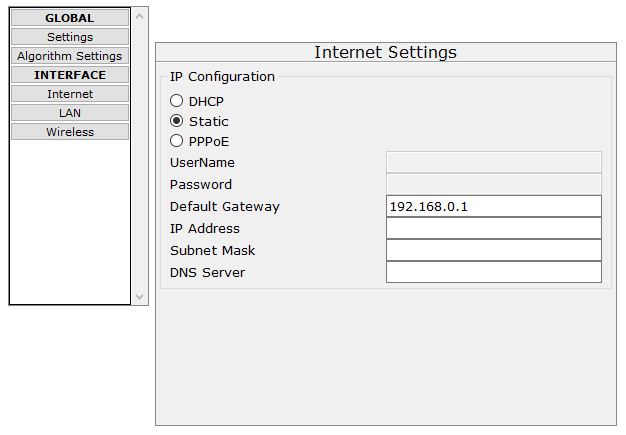
\includegraphics[width=\linewidth]{images/08.wireless/16.png}
\end{center}

Una volta finita anche quest’ultima operazione, la rete wireless potrà finalmente comunicare con tutte le altre reti, infatti se venisse configurata un'altra rete e venisse effettuato un ping da un dispositivo nella rete wireless verso uno in un'altra rete, la comunicazione avverrà con successo.

\begin{center}
    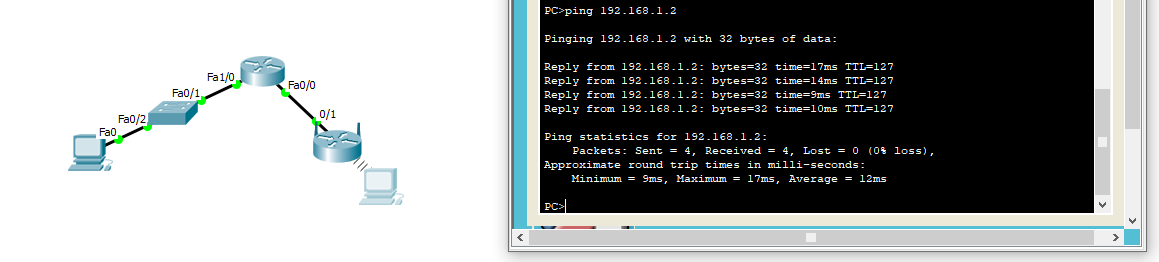
\includegraphics[width=\linewidth]{images/08.wireless/17.png}
\end{center}

\subsection{Reti wireless con server radius}
Prima di passare alla configurazione del server Radius dobbiamo capire cos’è di cosa si occupa.
Radius è l’acronimo di Remote Authentication Dial in User Service e serve per garantire sia l’accesso alla rete e sia la gestione degli account utente. Grazie all’implementazione del server Radius si riescono a garantire nella rete l’autenticazione, l’autorizzazione e l’accounting. 

\smallskip

Ora che abbiamo capito cos’è e a cosa serve il server radius vediamo come configurarlo.

\smallskip

Per prima cosa andiamo nel riquadro situato in basso a sinistra, clicchiamo su End Devices e aggiungiamo il server alla nostra rete già esistente.

Dopo di che il prossimo passaggio sarà quello di collegare il server alla porta LAN del Wireless Router.

Apriamo le impostazioni di configurazione del server facendo click su di esso, nel menù in alto selezioniamo

“Config” --> Fast Ethernet e inseriamo l’indirizzo IP dell’interfaccia.

Sempre nella stessa schermata nella parte alta troviamo la voce “Services”, entriamo e facciamo click sul servizio AAA che troviamo sul lato sinistro; una volta aperta la nuova scheda settiamo la Combo Box su ON per abilitare il server ad usare il servizio AAA.


\begin{center}
    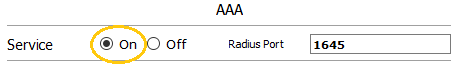
\includegraphics[width=\linewidth]{images/08.wireless/18.png}
\end{center}

Inseriamo i valori negli appositi spazi, quindi inseriamo il nome del client, l’indirizzo IP, la password e il tipo di server che vogliamo usare (nel nostro caso Radius); dopo di ciò facciamo click sul pulsante ADD per aggiungere la configurazione.


\begin{center}
    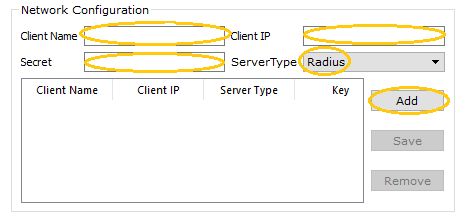
\includegraphics[width=\linewidth]{images/08.wireless/19.png}
\end{center}

Senza uscire dalla scheda corrente dobbiamo anche aggiungere tutti gli utenti che potranno accedere alla rete WI-FI, quindi inseriamo negli appositi spazi Username e Password e come prima facciamo click sul pulsante ADD per aggiungere quell’utente alla lista di utenti che potranno accedere alla rete wireless.

\begin{center}
    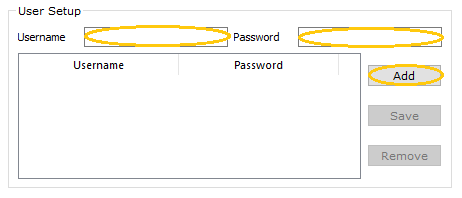
\includegraphics[width=\linewidth]{images/08.wireless/20.png}
\end{center}

La configurazione per quanto riguarda il Server Radius è finita, ora manca solo la configurazione degli host della rete per far sì che essi possano comunicare con il Server e richiedere l’accesso alla rete.

Per configurare un host rechiamoci nella sua scheda di configurazione, come fatto in precedenza anche per il Server Radius, selezioniamo WPA2 come metodo di autenticazione e inseriamo lo User ID, la password e selezioniamo TKIP come tipo di sicurezza.

\begin{center}
    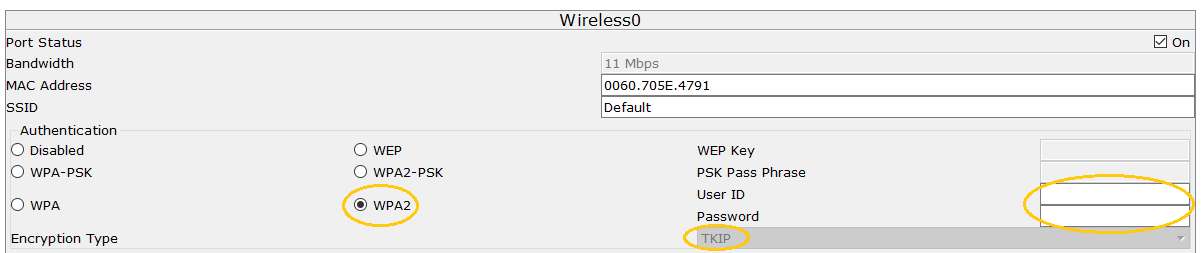
\includegraphics[width=\linewidth]{images/08.wireless/21.png}
\end{center}

Ora ci basta ripetere quest’ultima operazione per tutti gli host presenti sulla rete wireless e la nostra rete con Server Radius è pronta per essere utilizzata.